\documentclass[11pt]{report}

%-------------------------------------------------------------------------------------------------%

% PAQUETES

\usepackage[a4paper, right = 0.8in, left = 0.8in, top = 0.8in, bottom = 0.8in]{geometry}
\usepackage[utf8]{inputenc}
\usepackage[spanish]{babel}
\usepackage{amsmath,amsfonts,amssymb,amsthm}
\usepackage{multicol}
\usepackage{fouriernc}
\usepackage{enumitem}
\usepackage{mathtools} % Solo uso \underbracket
\usepackage{cellspace, tabularx, booktabs} % Líneas del título
\usepackage{parskip}
\usepackage{pdfpages}
\usepackage{cancel}

%-------------------------------------------------------------------------------------------------%

% AJUSTES GENERALES

\setlist[enumerate]{label={\textit{\alph*})}}

\makeatletter % Para quitar el espacio adicional que el paquete parskip añade al principio y al final de una demostración
\renewenvironment{proof}[1][\proofname]{\par
  \pushQED{\qed}%
  \normalfont \topsep\z@skip % <---- changed here
  \trivlist
  \item[\hskip\labelsep
        \itshape
    #1\@addpunct{.}]\ignorespaces
}{%
  \popQED\endtrivlist\@endpefalse
}
\makeatother

%-------------------------------------------------------------------------------------------------%

% COMANDOS PERSONALIZADOS

\newcommand{\N}{\mathbb N}
\newcommand{\Z}{\mathbb Z}
\newcommand{\Q}{\mathbb Q}
\newcommand{\R}{\mathbb R}
\newcommand{\C}{\mathbb C}

\newcommand{\pars}[1]{\left( #1 \right)} % Paréntesis de tamaño automático
\newcommand{\comment}[1]{}

%-------------------------------------------------------------------------------------------------%

% EJERCICIOS Y SOLUCIONES

\newtheorem{ejercicio}{Ejercicio}
\addto\captionsspanish{\renewcommand*{\proofname}{Solución}}

%-------------------------------------------------------------------------------------------------%

\begin{document}

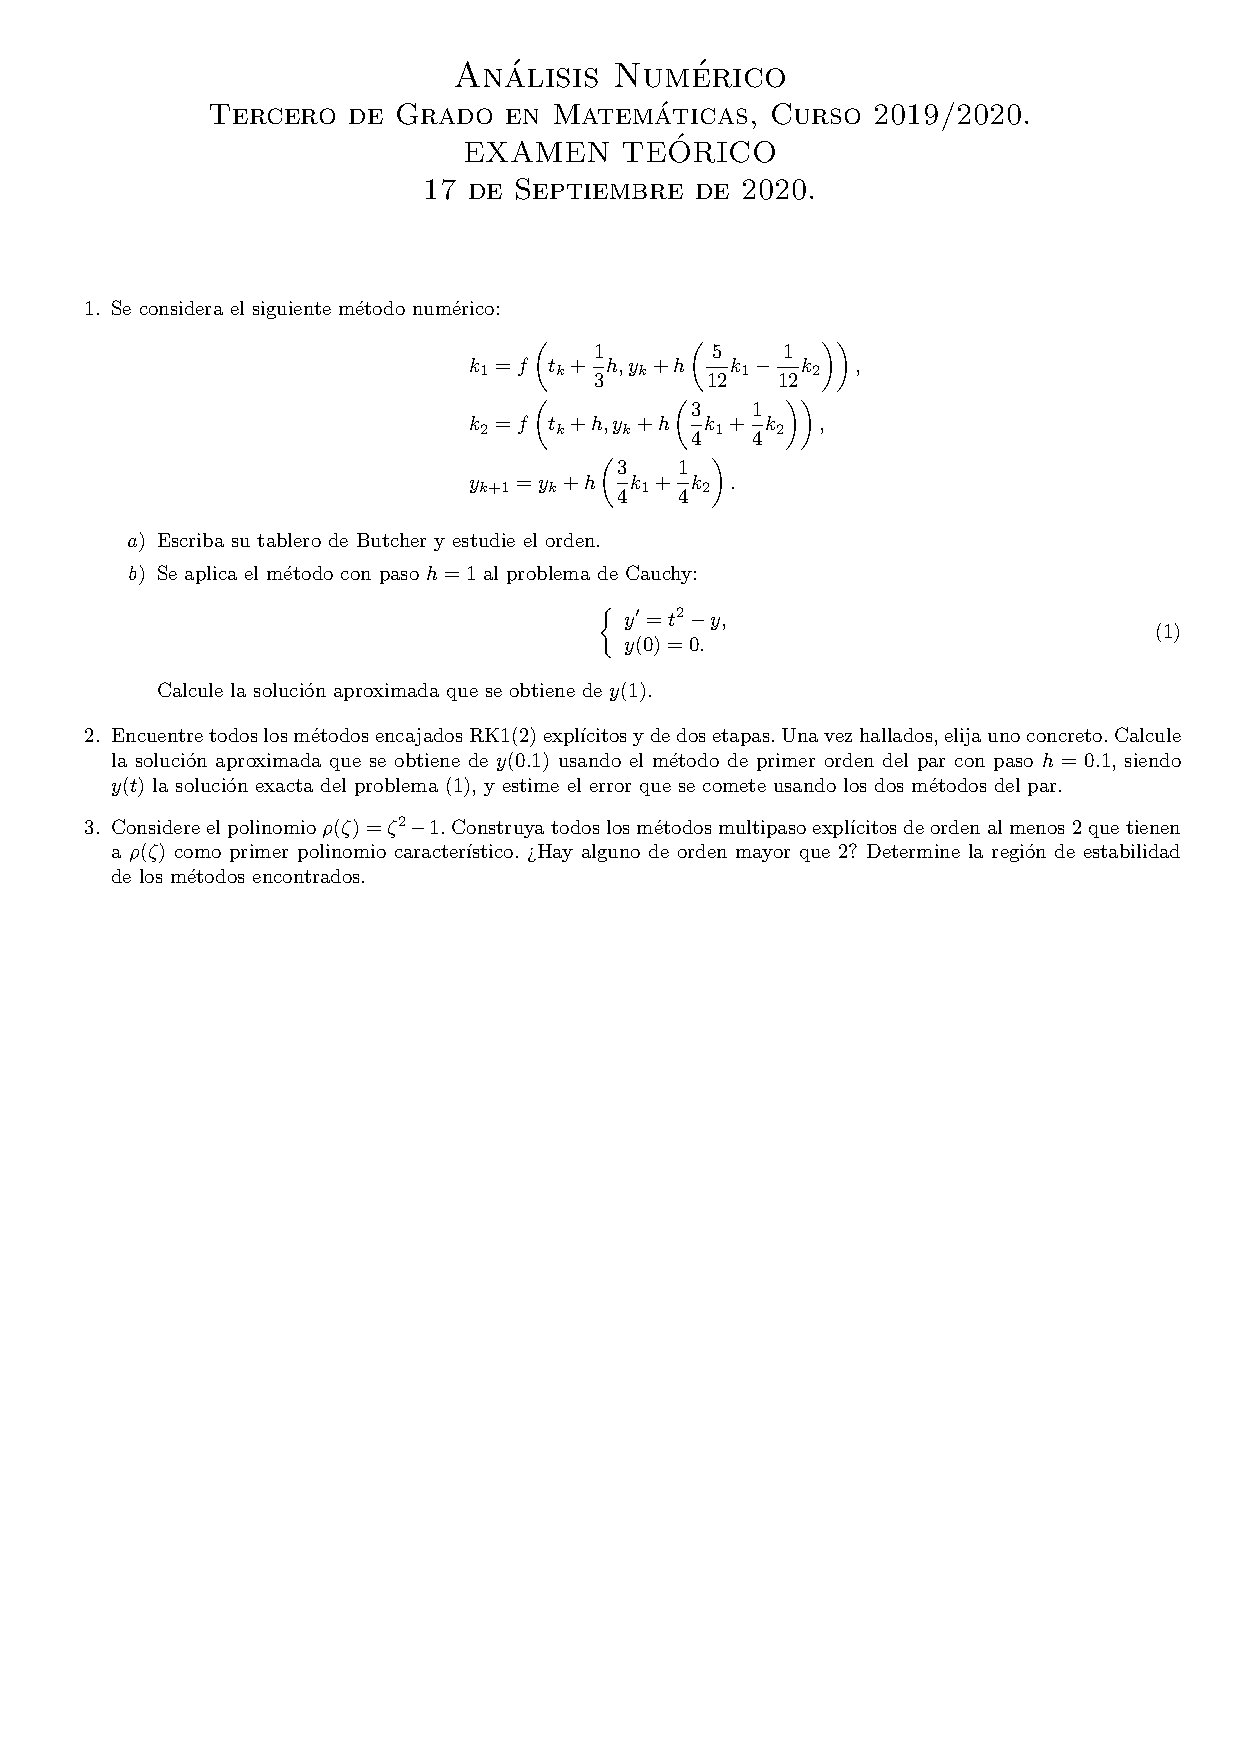
\includepdf[pages=-]{an_examen_2020-09.pdf}

%-------------------------------------------------------------------------------------------------%

% TÍTULO

\begin{center}

	\textbf{$-$ Resolución $-$}

\end{center}

%-------------------------------------------------------------------------------------------------%

\textbf{1.} 

\begin{enumerate}
    \item Sean
\[\textstyle y_k^{(1)} = y_k+h\bigl(\frac{5}{12}k_1-\frac{1}{12}k_2\bigr), \qquad \qquad y_k^{(2)} = y_k+h\bigl(\frac{3}{4}k_1+\frac{1}{4}k_2\bigr)\]
Entonces se tiene
\[\textstyle k_1 = f\bigl(t_k+\frac{1}{3}h,y_k^{(1)}\bigr), \qquad \qquad k_2 = f\bigl(t_k+h,y_k^{(2)}\bigr)\]
Por tanto, el método del enunciado puede escribirse como 
\[(RK) \ \begin{cases}
    y_k^{(1)}  &\hspace{-3mm}= y_k+h\bigl(\frac{5}{12}f\bigl(t_k+\frac{1}{3}h,y_k^{(1)}\bigr)-\frac{1}{12}f\bigl(t_k+h,y_k^{(2)}\bigr)\bigr)  \\[5pt]
    y_k^{(2)} &\hspace{-3mm}= y_k+h\bigl(\frac{3}{4}f\bigl(t_k+\frac{1}{3}h,y_k^{(1)}\bigr)+\frac{1}{4}f\bigl(t_k+h,y_k^{(2)}\bigr)\bigr) \\[5pt]
    y_{k+1} &\hspace{-3mm}= y_k+h\bigl(\frac{3}{4}f\bigl(t_k+\frac{1}{3}h,y_k^{(1)}\bigr)+\frac{1}{4}f\bigl(t_k+h,y_k^{(2)}\bigr)\bigr)
\end{cases}\]
El tablero de Butcher del método sería

\begin{center}
    \setlength\extrarowheight{2.5pt}
    \begin{tabular}{c|cc}
        1/3 & 5/12 & -1/12 \\
        1 & 3/4  & \phantom{-}1/4 \\ \hline
        & 3/4 & \phantom{-}1/4
    \end{tabular}
\end{center}

Sean
\[B = \left(\begin{array}{c}
    3/4 \\
    1/4
\end{array}\right) \qquad \qquad E = \left(\begin{array}{c}
    1 \\
    1
\end{array}\right) \qquad \qquad A = \left(\begin{array}{cc}
    5/12 & -1/12 \\
    3/4 & \phantom{-}1/4
\end{array}\right) \qquad \qquad C = \left(\begin{array}{cc}
    1/3 & 0 \\
    0 & 1
\end{array}\right) \]
En primer lugar,
\[B^tE = \left(\begin{array}{cc}
    3/4 & 1/4
\end{array}\right)\left(\begin{array}{c}
    1 \\
    1
\end{array}\right) = 1,\]
así que el método es de orden $1$. Como además
\[B^tAE = \left(\begin{array}{cc}
    3/4 & 1/4
\end{array}\right)\left(\begin{array}{cc}
    5/12 & -1/12 \\
    3/4 & \phantom{-}1/4
\end{array}\right)\left(\begin{array}{c}
    1 \\
    1
\end{array}\right) = \left(\begin{array}{cc}
    1/2 & 0
\end{array}\right)\left(\begin{array}{c}
    1 \\
    1
\end{array}\right) = 1\frac{1}{2}\]
Por tanto el método es de orden $2$. Y como
\[\begin{aligned}[t]
    B^tC^2E &= \left(\begin{array}{cc}
        3/4 & 1/4
    \end{array}\right)\left(\begin{array}{cc}
        1/3 & 0 \\
        0 & 1
    \end{array}\right)\left(\begin{array}{cc}
        1/3 & 0 \\
        0 & 1
    \end{array}\right)\left(\begin{array}{cc}
        1 \\
        1
    \end{array}\right)
= \left(\begin{array}{cc}
    1/4 & 1/4
\end{array}\right)\left(\begin{array}{c}
    1/3 \\
    1
\end{array}\right) = \frac{1}{12}+\frac{1}{4} = \frac{1}{3}, \\
B^tACE &= \left(\begin{array}{cc}
    3/4 & 1/4
\end{array}\right)\left(\begin{array}{cc}
    5/12 & -1/12 \\
    3/4 & \phantom{-}1/4
\end{array}\right)\left(\begin{array}{cc}
    1/3 & 0 \\
    0 & 1
\end{array}\right)\left(\begin{array}{cc}
    1 \\
    1
\end{array}\right)
= \left(\begin{array}{cc}
    1/2 & 0
\end{array}\right)\left(\begin{array}{c}
    1/3 \\
    1
\end{array}\right)
\end{aligned} = \frac{1}{6},\]
entonces el método es de orden $3$. Pero
\[B^tC^3E = \left(\begin{array}{cc}
    3/4 & 1/4
\end{array}\right)\left(\begin{array}{cc}
    1/3 & 0 \\
    0 & 1
\end{array}\right)^3\left(\begin{array}{cc}
    1 \\
    1
\end{array}\right)
= \left(\begin{array}{cc}
1/4 & 1/4
\end{array}\right)\left(\begin{array}{cc}
    1/3 & 0 \\
    0 & 1
\end{array}\right)\left(\begin{array}{c}
1/3 \\
1
\end{array}\right) = \frac{1}{36}+\frac{1}{4} = \frac{5}{18} \neq \frac{1}{4}\]
Concluimos que el orden del método es exactamente $3$.
\item Como $t_0 =0$, entonces $t_1 = h = 1$. Poniendo $h=1$, $k = 0$ e $y_0 = 0$ en el sistema $(RK)$,
\[\begin{cases}
    y_0^{(1)}  &\hspace{-3mm}=\frac{5}{12}f\bigl(\frac{1}{3},y_0^{(1)}\bigr)-\frac{1}{12}f\bigl(1,y_0^{(2)}\bigr)  \\[5pt]
    y_0^{(2)} &\hspace{-3mm}=\frac{3}{4}f\bigl(\frac{1}{3},y_0^{(1)}\bigr)+\frac{1}{4}f\bigl(1,y_0^{(2)}\bigr) \\[5pt]
    y_{1} &\hspace{-3mm}=\frac{3}{4}f\bigl(\frac{1}{3},y_0^{(1)}\bigr)+\frac{1}{4}f\bigl(1,y_0^{(2)}\bigr)
\end{cases}\]
Como en el problema $(1)$ es $f(t,y) = t^2-y$,
\[\begin{cases}
    y_0^{(1)}  &\hspace{-3mm}=\frac{5}{12}\bigl(\frac{1}{9}-y_0^{(1)}\bigr)-\frac{1}{12}\bigl(1-y_0^{(2)}\bigr) = -\frac{1}{27}-\frac{5}{12}y_0^{(1)}+\frac{1}{12}y_0^{(2)} \\[5pt]
    y_0^{(2)} &\hspace{-3mm}=\frac{3}{4}\bigl(\frac{1}{9}-y_0^{(1)}\bigr)+\frac{1}{4}\bigl(1-y_0^{(2)}\bigr) =\frac{1}{3}-\frac{3}{4}y_0^{(1)}-\frac{1}{4}y_0^{(2)} \\[5pt]
    y_{1} &\hspace{-3mm}=y_0^{(2)}
\end{cases}\]
De la primera ecuación se obtiene
\[y_0^{(1)} = \frac{-\frac{1}{27}+\frac{1}{12}y_0^{(2)}}{1+\frac{5}{12}} = \frac{12}{17}\left(-\frac{1}{27}+\frac{1}{12}y_0^{(2)}\right) = -\frac{4}{153}+\frac{1}{17}y_0^{(2)}\]
Sustituyendo en la segunda,
\[y_0^{(2)} = \frac{1}{3}-\frac{3}{4}\left( -\frac{4}{153}+\frac{1}{17}y_0^{(2)}\right)-\frac{1}{4}y_0^{(2)} = \frac{1}{3}+\frac{1}{51}-\frac{3}{68}y_0^{(2)}-\frac{1}{4}y_0^{(2)} = \frac{6}{17}-\frac{5}{17}y_0^{(2)}\]
De esto se deduce que
\[y(1) \approx y_1 = \frac{\frac{6}{17}}{1+\frac{5}{17}} = \frac{17}{22} \cdot \frac{6}{17} = \frac{3}{11}\]
\end{enumerate}

\textbf{2. } De encajados nada.

\textbf{3. } Los métodos multipaso con polinomio caractersítico $\rho(\zeta) = \zeta^2-1$ son de la forma
\[y_{k+2}-y_k = h\bigl(\beta_2f_{k+2}+\beta_1f_{k+1}+\beta_0f_k\bigr)\]
Los que son explícitos deben tener $\beta_2 = 0$, así que
\[y_{k+2}-y_k = h\bigl(\beta_1f_{k+1}+\beta_0f_k\bigr) \tag{$\ast$}\]
Estudiemos el orden de un método de esta forma. Se tiene que
\[\sum_{j=0}^2 \alpha_j = 0, \qquad \qquad \sum_{j=0}^2 \alpha_jj = 2, \qquad \qquad \sum_{j=0}^2\beta_j = \beta_0 +\beta_1,\]
así que el método es de orden $1$ si y solo si $\beta_0+\beta_1 = 2$. Además,
\[\sum_{j=0}^2\alpha_jj^2 = 4, \qquad \qquad 2\sum_{j=0}^2 \beta_jj = 2\beta_1,\]
así que el método es de orden $2$ si y solo si $\beta_0+\beta_1 = 2$ y $2\beta_1 = 4$, es decir, si y solo si $\beta_1 = 2$ y $\beta_0 = 0$. Así, el único método multipaso de la forma $(\ast)$ de orden al menos $2$ es
\[y_{k+2}-y_k = 4hf_{k+1}\]
Y como
\[\sum_{j=0}^2 \alpha_jj^3 = 8, \qquad \qquad 3\sum_{j=0}^2 \beta_jj^2 = 3 \cdot 4 = 12 \neq 8,\]
entonces el método no es de orden $3$. Hallemos la frontera de la región de estabilidad, que es
\[\partial D_A = \{\hat{h} \in \C \colon \pi_{\hat{h}} \textup{ tiene alguna raíz de módulo } 1\},\]
donde $\pi_{\hat{h}}(z)=\rho(z)-\hat{h}\sigma(z)=z^2-1-4\hat{h}z$. Se tiene que
\[\pi_{\hat{h}}(z)=0 \iff \hat{h} = \frac{z^2-1}{4z}\]
Nótese que $z \neq 0$ porque $0$ no es raíz de $\pi_{\hat{h}}$. Además, si $\hat{h} \in \partial D_A$, entonces $\pi_{\hat{h}}$ tiene alguna raíz de módulo $1$, que es de la forma $e^{i\theta}$ para algún $\theta \in \R$. Por tanto,
\[\hat{h}=\frac{e^{2i\theta}-1}{4e^{i\theta}} = \frac{1}{4}e^{i\theta} - \frac{1}{4}e^{-i\theta} = \frac{1}{4}2i\sen \theta = \frac{1}{2}i\sen \theta\]
Como $|\frac{1}{2}\sen\theta| \leq \frac{1}{2}$, Esto nos dice que
\[\partial D_A \subset \left\{iy  \in \C \colon -\frac{1}{2} \leq y \leq \frac{1}{2}\right\}\]
En otras palabras, $\partial D_A$ es un segmento del eje imaginario, así que hay dos opciones: $D_A = \C \setminus \partial D_A$ o $D_A = \emptyset$. Lo primero no puede darse porque $D_A$ no contiene al eje real positivo en algún entorno del origen, luego debe ser $D_A = \emptyset$.
\end{document}